
\documentclass[a4paper,fleqn]{cls/cas-dc}


\usepackage[numbers]{natbib}



\begin{document}
\let\WriteBookmarks\relax
\def\floatpagepagefraction{1}
\def\textpagefraction{.001}
\shorttitle{Jan Luecker, Christian S. Fischer / Two-flavor QCD at finite temperature and chemical potential in a functional approach}
\shortauthors{Jan Luecker}

\title [mode = title]{Two-flavor QCD at finite temperature and chemical potential in a functional approach}                      


\author[1]{Jan Luecker}[type=editor,
                        orcid=0000-0001-7511-2910 ]
\cormark[1]
\ead{Jan.Luecker@theo.physik.uni-giessen.de}

\address[1]{Institut f{\"u}r Theoretische Physik, Justus-Liebig-Universit{\"a}t Gie{\ss}en, Heinrich-Buff-Ring 16, D-35392 Gie{\ss}en, Germany}

\author[1,2]{Christian S. Fischer}

\address[2]{GSI Helmholtzzentrum f{\"u}r Schwerionenforschung GmbH, Planckstr., 1 D-64291 Darmstadt, Germany}

\cortext[cor1]{Corresponding author}

\begin{abstract}
We summarize recent results obtained in the Dyson-Schwinger formalism to study
the chiral and deconfinement phase transitions of quenched and unquenched QCD at
finite temperature and chemical potential. In the quenched case we compare SU(2)and
SU(3)gauge theories by taking lattice data for the gluon as an input for the quark
Dyson–Schwinger equation. As compared to previous investigations we find a clearer
distinction between the second order transition of the two-color theory and the (weak) first
order transition of the three-color gauge theory. We then extend this study to unquenched
QCD at finite chemical potential by taking matter effects to the gluon into account and
investigate the order of the chiral phase transition and the behavior of the deconfinement
transition. What we find are coinciding phase transitions up to a critical endpoint which is
located at large chemical potential.

\rightline{$\copyright$ 2012 Elsevier B.V. All rights reserved.}
\end{abstract}

\begin{keywords}
Dyson–Schwinger equations \sep 
QCD phase diagram \sep 
Confinement \sep 
Chiral symmetry breaking
\end{keywords}


\maketitle

\section{Introduction}

The behavior of quantum chromodynamics at large temperatures and densities received a lot of attention over the past
years and is an ongoing research program from both, the theoretical and experimental side. At vanishing chemical potential
lattice QCD has shown the existence of a crossover from the chiral symmetry broken and confined hadronic phase to the
phase of the (approximately) chiral symmetric and deconfined quark-gluon plasma. While this has been confirmed many
times, the behavior at finite chemical potential is still under intense debate. Lattice methods have a limited applicability
here due to the fermion sign problem.

Models like the Nambu-Jona-Lasinio (NJL) and the quark-meson (QM) model have so far been the main source of
studies at large chemical potential, and established a scenario where the chiral crossover turns into a first order phase
transition at a critical endpoint. In Polyakov loop extended versions these models (PNJL and PQM) have also been used to
study the confinement/deconfinement transition, which may or may not coincide with the chiral transition \cite{HERBST201158,PhysRevD.73.014019,PhysRevD074023,PhysRevC.83.054904}. At large
chemical potentials and relatively small temperatures there may also exist some new phases, e.g.\ color superconductors,
inhomogeneous \cite{KOJO201037,PhysRevLett.103.072301} or quarkyonic \cite{MCLERRAN200783} phases.

Another direct approach to non-perturbative QCD without the sign problem is the framework of Dyson-Schwinger
equations (DSEs) \cite{PhysRevLett.103.052003,FISCHER2011438,Fischer2010} and the functional renormalization group \cite{BRAUN2010262,PhysRevLett.106.022002}. QCD with two degenerate quark flavors has
been studies in Ref. \cite{FISCHER2011438} by solving the coupled system of quark and gluon DSEs using quenched lattice data for the gluon
propagator as input. Within this truncation scheme the behavior of the chiral and deconfinement transitions at finite
chemical potential have been investigated using the first calculation of the dressed Polyakov loop in this region of the QCD 
phase diagram. In this proceedings contribution we give an overview of the employed truncation scheme and summarize
the corresponding results.

\section{Order parameters for chiral symmetry breaking and confinement}
The central object of our investigations is the in-medium quark propagator which can be decomposed as
\begin{equation}
	S^{-1}(p) = i \vec{\gamma} \vec{p} A(\omega_n, \vec{p}^2) + i \gamma_4(\omega_n + i\mu)C(\omega_n, \vec{p}^2) + B(\omega_n,\vec{p}^2) ,
\end{equation}
where $\mu$ is the quark chemical potential and $\omega_n = \pi T( 2n + 1 )$ are the Matsubara modes in the imaginary time formalism
with temperature $T$. The functions $A$, $C$ and $B$ dress the vector and scalar part of the propagator which we calculate from the
corresponding DSE. The bare propagator $S_0$ at quark mass $m$ is characterized by $A = C = 1$ and $B = m$. A quark propagator
with a non-vanishing $B$ function corresponds to a phase of broken chiral symmetry, either explicitly by a bare quark mass
or dynamically by quantum effects.

A possible order parameter for chiral symmetry breaking is the quark condensate
\begin{equation}
\begin{split}
	&\langle \overline{\psi} \psi \rangle = \text{Tr}[S] = Z_2 Z_m T \cdot \\
	&\sum_n \int \frac{d^3}{(2 \pi)^3} \frac{4 \cdot B(\omega_n, \vec{p}^2)}{\vec{p}^2 A^2(\omega_n, \vec{p}^2) + \omega_n^2 C^2(\omega_n, \vec{p}^2) + B^2(\omega_n, \vec{p}^2)},
	\end{split}
\end{equation}
which can be calculated directly from a solution of the quark DSE. The condensate in this definition is divergent with $m \Lambda^2$
and $m^2 \Lambda$ , but since these terms do not depend on temperature and chemical potential the condensate can still be used as
an order parameter. We work with approximately physical quark masses and therefore expect to find a crossover at small
chemical potentials. To define the pseudo-critical temperature in this case we use the susceptibility
\begin{equation}
	\chi = \frac{\partial \langle \overline{\psi}\psi \rangle}{\partial m},
\end{equation}
and determine its maximum to find $T_c$ . The divergent terms in the condensate only lead to an offset in $\chi$, without changing
its maximum. The quark condensate in the chiral limit has been determined in Ref. \cite{PhysRevD.84.054013}, where critical scaling beyond the
mean field level at the second order chiral phase transition has been studied.

Constructing an order parameter for confinement that is accessible with functional methods is a more challenging task.
In the quenched case the Polyakov loop is an accepted order parameter which is known to show a (weak) first order phase
transition for QCD at a temperature of approximately 270 MeV and a second order transition for the two-color gauge theory
at approximately 300 MeV. The Polyakov-loop expectation value is sensitive to breaking of center symmetry, which occurs in
the deconfined phase, while the confined phase is center symmetric. However, if finite quark masses are taken into account
within QCD, center symmetry is broken explicitly (just like chiral symmetry). There are, however, interesting indications
that this might not be the case if the larger center symmetry of the full standard model is taken care of.

In \cite{PhysRevD.77.094007,PhysRevLett.97.032003,PhysRevD.75.114003} the so-called dual condensates have been proposed as order parameters for center symmetry breaking. They
are defined as
\begin{equation}
	\Sigma_n = \int_{0}^{2\pi} \frac{d \varphi}{2 \pi} e^{-i \varphi n} \langle \overline{\psi}\psi \rangle_\varphi,
\end{equation}
where $\varphi \in [ 0 , 2\pi ]$ is a parameter for $U (1 )$-valued boundary conditions of the quark fields: $\psi(\vec{x} , 1 / T ) = e^{i\varphi} \psi(\vec{x} , 0 )$. The
physical boundary condition is $\varphi = \pi$. The quantity $\Sigma_n$ contains all loops of connections winding $n$ times around the
Euclidean time direction. For $n = ± 1$ this also contains the Polyakov loop, and $\Sigma_{\pm 1}$ has therefore been named the 'dressed
Polyakov loop’. It also contains all kinds of loops which are not straight in the time direction but contain detours, but these
loops are $1 / m$ suppressed. In the $m \rightarrow \infty$ limit the normal Polyakov loop is recovered. At finite chemical potential $\Sigma_{+1}$
and $\Sigma_{- 1}$ are not equal and correspond to the dressed Polyakov loop and its conjugate. Since the dressed Polyakov loop is
sensitive to center symmetry breaking, it allows us to calculate the confinement/deconfinement transition from solutions of
the quark DSE without having to deal with an ansatz for a Polyakov-loop potential as necessary in the PNJL and PQM models.


Since the deconfinement transition will be a crossover in the unquenched case, we use the maximum of $\frac{\partial \Sigma_{\pm 1}}{\partial m} $ to define
the pseudo-critical temperature, similar to the chiral transition.

	\begin{figure*}
	\centering
	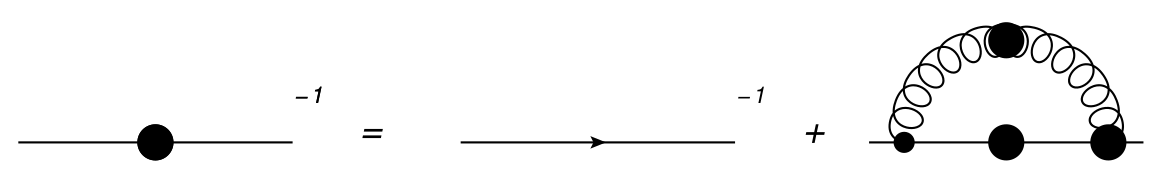
\includegraphics[width=\textwidth,height=1.4in]{fig/fig1.png}
	\caption{The Dyson-Schwinger equation for the quark propagator. Dots denote dressed objects.}
	\label{FIG:1}
\end{figure*}
\begin{figure*}
	\centering
	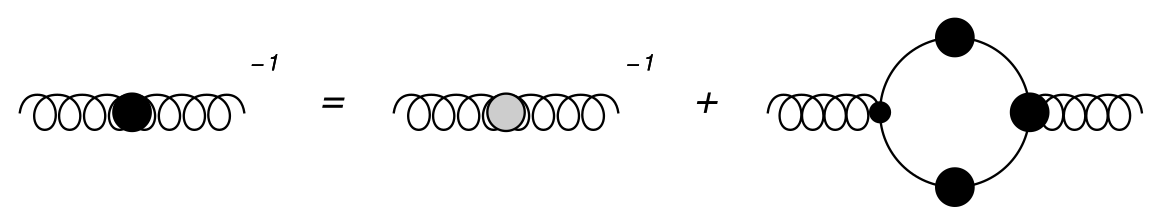
\includegraphics[width=\textwidth,height=1.3in]{fig/fig2.png}
	\caption{The truncated gluon DSE. The black dot denotes the full, unquenched propagator, while the gray dot denotes the quenched propagator.}
	\label{FIG:2}
\end{figure*}
\section{Dyson-Schwinger equations}
Fig.\ref{FIG:1} displays the DSE for the quark propagator. The quark self-energy depends on the fully dressed gluon and quark-gluon vertex, which we need to specify in order to solve the equation self-consistently. For the in-medium gluon
propagator we take two steps, first we investigate quenched QCD where lattice calculations are up to now the most reliable
source for the temperature dependent gluon propagator, and then we will introduce unquenching effects by resorting to
the gluon DSE.

The unquenched gluon DSE in the truncation we use here is depicted in Fig. \ref{FIG:2}. The full propagator is given by the lattice
results for the quenched propagator and the quark loop. This is only an approximation, since all diagrams where quark
oops appear inside the Yang-Mills part of the self-energy are neglected. In vacuum this leads to an over-estimation of the
quark loop on the few percent level. Assuming this still holds at finite temperature, we expect to underestimate the critical
temperatures by up to 10 MeV.

The quark loop shown in Fig.\ref{FIG:2} is given by
\begin{equation}
	\Pi_{\mu \nu} (p) = \frac{Z_{1F} N_f}{2} \sum_n \int \frac{d^3 k}{(2 \pi)^3}\text{Tr}[S(q) g \gamma_\mu S(k) g \Gamma_\nu],
\end{equation}
where $q = p + k$ , $Z_{1F}$ is the vertex renormalization factor and $\Gamma_\mu$ the full quark-gluon vertex. In principle the system of
quark and gluon DSEs can now be solved self-consistently but as a first approximation we will treat the quark loop semi-
perturbatively by taking bare quarks but a dressed vertex. This allows us to use the hard-thermal loop expression multiplied
by the vertex dressing function, defined below. The HTL approximation is well justified above the critical temperature where
quark dressing effects are small, but needs to be corrected in the chiral broken phase. A calculation with a fully dressed quark
loop is work in progress.

Finally we have to specify our choice of the quark–gluon vertex, which appears in the quark self-energy and in the quark
loop. We use the same construction as in \cite{Fischer2010}. It is given by
\begin{equation}
\begin{split}
	&\Gamma_\mu(p, k; q) = \gamma_\mu \cdot \Gamma(p^2, k^2, q^2) \cdot \\
	& \left(\delta_{\mu, 4} \frac{C(p) + C(q)}{2} + \delta_{\mu, i} \frac{A(p) + A(q)}{2}\right),
	\end{split}
	\end{equation}\begin{equation}
	\begin{split}
	&\Gamma(p^2, k^2; q^2) = \\ 
	&\frac{d_1}{d_2 + q^2} + \frac{q^2}{\Lambda^2 + q^2}\left(\frac{\beta_0 \alpha(\nu) \ln [q^2 / \Lambda^2 + 1]}{4 \pi}\right)^{2 \delta}.
	\end{split}
\end{equation}
	In the $UV$ resummed perturbation theory is recovered with $\beta_0 = ( 11N_c - 2N_f )/ 3 , \alpha_\mu = 0.3 , \delta = - 9N_c /( 44N_c - 8N_f )$ and
	the scale $\Lambda = 1.4\text{GeV}$, which is inherited from the lattice gluon. In the IR we have two parameters, $d_1$ and $d_2$, which have
	been fixed to $d_2 = 0.5 \text{GeV}^2$ and $d_1 = 7.6 \text{GeV}^2$ for $SU(2)$ and $d_1 = 4.6 \text{GeV}^2$ for $SU(3)$.
	\begin{figure*}
		\centering
		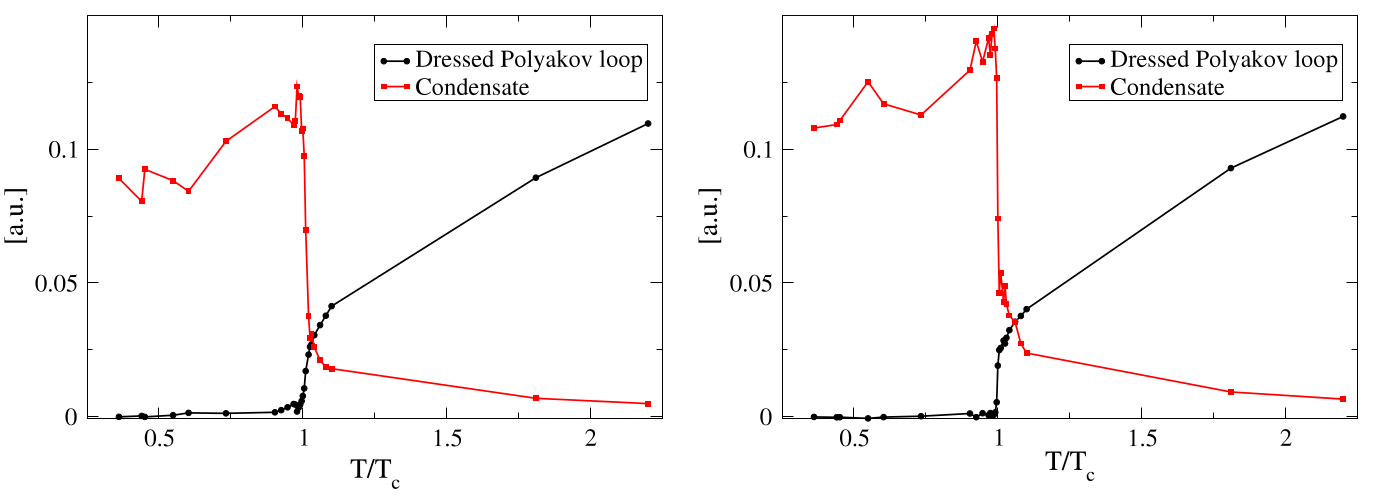
\includegraphics[width=\textwidth,height=2.5in]{fig/fig3.png}
		\caption{Dressed Polyakov loop and quark condensate for $SU ( 2 )$ (left) and $SU ( 3 )$ (right).}
		\label{FIG:3}
	\end{figure*}
	\begin{figure}
		\centering
		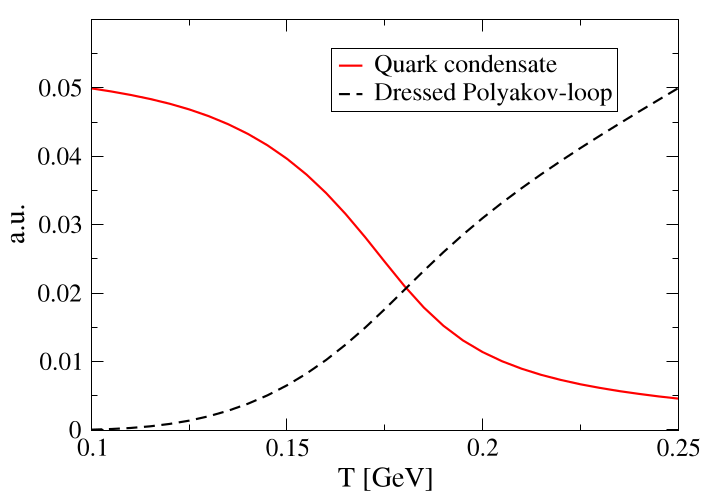
\includegraphics[width=3.4in,height=2.5in]{fig/fig4.png}
		\caption{Dressed Polyakov loop and quark condensate in two-flavor QCD as function of temperature at zero chemical potential.}
		\label{FIG:4}
	\end{figure}
	\begin{figure}
		\centering
		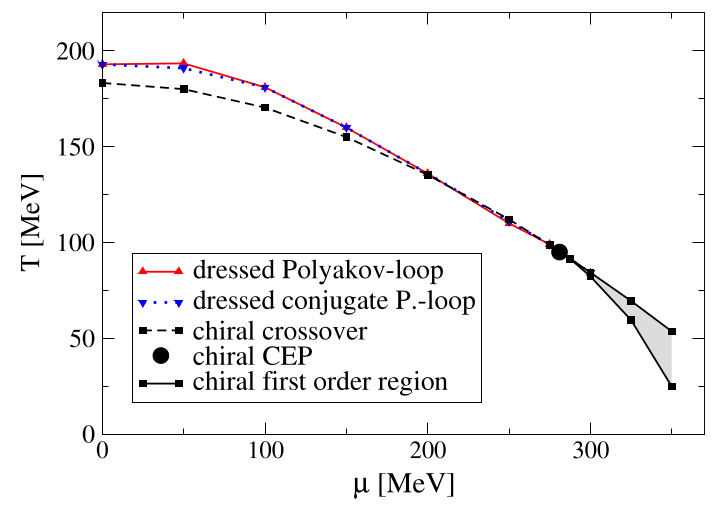
\includegraphics[width=3.3in,height=2.5in]{fig/fig5.png}
		\caption{The phase boundary for chiral symmetry and confinement at real chemical potential. The solid lines above the CEP denote the spinodals which
			mark the area of coexistence of chiral symmetric and broken solutions of the DSE.}
		\label{FIG:5}
	\end{figure}	
\section{Results}
\subsection{Quenched QCD}
As already mentioned above, the phase transition of quen-ched QCD (i.e.\ without the quark-loop contributions in the
Yang-Mills sector) can be determined from the quark DSE using quenched lattice data for the temperature dependent
gluon propagator as input. Of course, the quality of the results then depends on the statistic and systematic error of the
lattice. Starting from the pioneering work of Ref. \cite{PhysRevD.75.076003}, these have been improved in \cite{Fischer2010} and analyzed in more detail in recent
works. In general, however, it seems fair to say that in particular systematic errors due to volume and discretization
artifacts at small momenta are not yet well under control. This is particularly true in the vicinity of the critical temperature.
Consequently, it proved difficult to distinguish the order of the phase transition between the two-color and three-color cases
investigated in Ref. \cite{Fischer2010}. Here we present updated and improved results for the quark condensate and the dressed Polyakov
loop using the high-statistics lattice data of Ref. as input, which are also carried out on a much finer temperature grid
than the ones of \cite{Fischer2010}.

Fig.\ref{FIG:3} shows how the dressed Polyakov loop and the quark condensate change with temperature in the cases of two
and three colors. For the normalization of the temperature scale we use the transition temperatures which have been
determined from the Polyakov loop on the lattice and compare with our results obtained from the quark DSE. Indeed, both
order parameters show a rapid change at $T_c$ , signaling the (approximate) restoration of chiral symmetry and breaking of
center symmetry at the very same temperature in agreement with the critical temperature determined from the lattice.
With the finer temperature grid and the better statistics compared to \cite{Fischer2010}, the behavior of the dressed Polyakov loop is now
clearly distinguishable between the $SU ( 2 )$ and $SU ( 3 )$ cases, pointing towards a second order phase transition for $SU ( 2 )$ and
a weak first order for $SU ( 3 )$, again in agreement with the expectations. The situation is less clear for the chiral transition,
although also here we observe a steeper fall for the $SU ( 3 )$-case. The behavior of the quark condensate for temperatures
below the critical one, i.e.\ the rise with temperature combined with the sharp drop at T c has also been seen in quenched
lattice calculations \cite{PhysRevD.78.074505}. Nevertheless, it may very well be that the quantitative aspects of this rise are subject to the
systematic uncertainties of the lattice gluon data. These uncertainties are also reflected in the 'noisy' behavior of the
quark condensate. Nevertheless it is remarkable that below $T_c$ the dressed Polyakov loop is consistent with zero, signaling
conserved center symmetry.

\subsection{Unquenched QCD at finite temperature and chemical potential}
We now include two flavors of quarks via the quark loop as explained above. The effect of the matter sector on the
gluon is a reduction of the dressing functions, which leads to a reduced interaction strength in the quark self-energy, and
therefore to a smaller critical temperature. In Fig.\ref{FIG:4} we show the evolution of the order parameters at $\mu = 0$. What we
find is a crossover for both the condensate and the dressed Polyakov loop. The value for the pseudo-critical temperature is
$T_c^{N_f = 2} = 180 \pm 5 \text{ MeV}$ from the quark condensate and 
$T_c^{N_f = 2} = 195 \pm 5 \text{ MeV}$ from the dressed Polyakov loop. The difference
in these numbers can be attributed to the crossover nature of the transition.

When we go to $\mu > 0$ the condensate for neither periodic ($\varphi = 0$) nor anti-periodic ($\varphi = \pi$ ) boundary conditions
becomes complex. This leads to a difference in $\Sigma_{+1}$ and $\Sigma_{- 1}$, i.e.\ in the dressed Polyakov loop and its conjugate. In Fig.\ref{FIG:5} the
resulting phase diagram of two-flavor QCD is shown. For the chiral transition we observe a crossover up to relatively large
values of the chemical potential where we find a critical endpoint at ($T_{ EP}, \mu_{EP}) \approx ( 95 , 280 ) \text{ MeV}$. Since $\mu_{EP} / T_{EP} \approx 3 \gg 1$,
this result suggests that the CEP is outside the reach of lattice QCD. For the confinement/deconfinement transition we
observe that the critical temperature extracted from the dressed Polyakov loop and its conjugate is nearly equal, and close
to that extracted from the quark condensate. As the chemical potential is increased the crossover becomes steeper and the
two transition lines come closer together, meeting at around $\mu \approx 200 \text{ MeV}$.

Both results, the CEP at large $\mu$ and the coinciding phase transitions agree well with results from the PQM model \cite{PhysRevC.83.054904}
beyond mean field, where the matter back-reaction on the Yang-Mills sector is also taken into account.

We should note here that at the chemical potentials where we find the CEP our truncation scheme becomes less reliable,
since the influence of Baryons is neglected. It may therefore be advised to rephrase our results as an exclusion of the CEP
in the $\mu/ T < 1$ region. This is consistent with longstanding predictions from investigations of the curvature of the chiral
critical surface in the Columbia plot \cite{DEFORCRAND2002290} and also with recent lattice results on the curvature of the chiral and deconfinement
crossover lines at small chemical potential.

\section{Conclusion}
We have presented a truncation scheme for the Dyson-Schwinger equations of QCD where we take data from a lattice
calculation for the temperature dependent quenched gluon, and introduce the quark loop for studies of unquenched QCD,
namely at finite chemical potential.

Within this truncation we investigated the behavior of the quark condensate as an order parameter for chiral symmetry
breaking, and of the dressed Polyakov loop as an order parameter for confinement. In the quenched case at $\mu = 0$ we
found that the order parameters reproduce the lattice input, hinting at a second order phase transition for $SU ( 2 )$ and a
first order phase transition for $SU ( 3 )$ . At finite density we found that thermal fluctuations from the matter sector lead to
a critical endpoint at large densities while chiral and deconfinement transitions coincide. Our results serve as a basis for
further studies of hot and dense QCD.

\section*{Acknowledgments}
We are grateful to Jens A. Mueller for collaboration on part of the results summarized here. This work has been supported
by the Helmholtz Young Investigator Grant VH-NG-332 and the Helmholtz International Center for FAIR within the LOEWE
program of the State of Hesse.


\bibliographystyle{cls/cas-model2-names}

\bibliography{bib/cas-refs}

\end{document}

